\documentclass{pracamgr}
\usepackage{polski}
\usepackage{amssymb}
\usepackage{amsthm}
\usepackage{amsmath}
\usepackage{algorithmic}
\usepackage{algorithm}
\usepackage{pdfpages}
\usepackage{sistyle}
\usepackage[utf8]{inputenc}
\usepackage[pdfborder={0 0 0}]{hyperref}

\SIdecimalsign{,}
%include ps
\usepackage{graphicx}
%\epstopdfsetup{update}
%\DeclareGraphicsExtensions{.ps}
%\epstopdfDeclareGraphicsRule{.ps}{pdf}{.pdf}{ps2pdf -dEPSCrop -dNOSAFER #1 \OutputFile}


% Dane magistranta:

\author{Paweł Stawicki}
\nralbumu{189254}

\title{Wyznaczanie pozycji oraz orientacji w przestrzeni za pomocą ultradźwięków}
\tytulang{Determining position and orientation in space using ultrasound}

\kierunek{Informatyka}
\opiekun{dra inż. Marcina Peczarskiego}

\date{Wrzesień 2015}

%Podać dziedzinę wg klasyfikacji Socrates-Erasmus:
\dziedzina{ 
%11.0 Matematyka, Informatyka:\\ 
%11.1 Matematyka\\ 
%11.2 Statystyka\\ 
11.3 Informatyka\\ 
%11.4 Sztuczna inteligencja\\ 
%11.5 Nauki aktuarialne\\
%11.9 Inne nauki matematyczne i informatyczne
}

%Klasyfikacja tematyczna wedlug AMS (matematyka) lub ACM (informatyka)
%\klasyfikacja{D. Software\\
%  D.127. Blabalgorithms\\
%  D.127.6. Numerical blabalysis}
\klasyfikacja{
TODO: dodać
%I.4.8 Scene Analysis, Subject: Tracking
%B.0 [Hardware]: General
%B.4 [Hardware]: Input/Output & Data Communication 
%H.4.m [Information Systems Applications]: Mis-
%cellaneous
}

% S?owa kluczowe:
\keywords{położenie, lokalizacja, orientacja, 3D, ultradźwięki}

\renewcommand{\algorithmicrequire}{\textbf{Input:}}
\renewcommand{\algorithmicensure}{\textbf{Output:}}
\renewcommand{\algorithmiccomment}[1]{// #1}

% Tu jest dobre miejsce na Twoje w?asne makra i ?rodowiska:
\newtheorem{defi}{Definicja}[section]
\newtheorem*{ndefi}{Definicja}
\newtheorem{theorem}{Twierdzenie}[section]

\newcommand{\V}[1]{\ensuremath{\mathbf{#1}}}
\newcommand{\T}[1]{\ensuremath{ {#1}^{\mathbf{{T}}}}}
\newcommand{\Tnawiasy}[1]{\ensuremath{ ({#1})^{\mathbf{{T}}}}}
\newcommand{\M}[1]{\ensuremath{\mathbf{#1}}}
\newcommand{\Sp}[1]{\ensuremath{\mathcal{#1}}}
\newcommand{\SpG}[1]{\ensuremath{\langle {#1} \rangle }}
\newcommand{\cialo}[1]{\ensuremath{\mathcal{#1}}}

\newcommand{\nxn}{\ensuremath{ n \times n }}

\newcommand{\prodA}[2]{\ensuremath{ \langle #1 , #2 \rangle_{\M{A}}}}
\newcommand{\prodAA}[2]{\ensuremath{ \T{#1} \M{A} #2 }}
\newcommand{\prodAATnawiasy}[2]{\ensuremath{ \Tnawiasy{#1} \M{A} #2 }}
\newcommand{\dsum}{\displaystyle\sum}

\newcommand{\Axmb}{ \M{A} \V{x} - \V{b}}
\newcommand{\Adxmb}{ \M{A} \V{\dot{x}} - \V{b}}
\newcommand{\dx}{\ensuremath{\dot{\V{x}}}}

%rzutowanie (projekcja)
\newcommand{\projA}[2]{\ensuremath{ {proj_{#1} (#2)   }}}
\newcommand{\projAWzor}[2]{\ensuremath{ {\displaystyle\frac{\prodA{#1}{#2}}{ \prodA{#1}{#1}}  #1 }}}
\newcommand{\projAWzorM}[2]{\ensuremath{#1 ( \prodAA{#1}{#1} )^{-1} \T{#1} \M{A} #2 }}
\newcommand{\projAWzorMTnawiasy}[2]{\ensuremath{#1 ( \prodAATnawiasy{#1}{#1} )^{-1} \Tnawiasy{#1} \M{A} #2 }}

\newcommand{\Winv}[1]{\ensuremath{ \M{W}_{#1}^{\mathtt{inv}} }}

\newcommand{\rank}[1]{\ensuremath{ rank(#1)}}
\newcommand{\Zdwa}{\ensuremath{ \mathbb{Z}_2}}
\newcommand{\Zdwan}{\ensuremath{ {\displaystyle\mathbb{Z}_2^n}}}

\newcommand{\AWSTV}[1]{\ensuremath{\M{A}\M{W}_{#1} \T{\M{S}_{#1}} + \M{V}_{#1} }}
\newcommand{\VWinvVT}[1]{\ensuremath{\M{V}_{#1} \Winv{#1} \T{\M{V}_{#1}}  }}
\newcommand{\VTAVWinv}[1]{\ensuremath{\T{\M{V}_{#1}} \M{A} \M{V}_{#1} \Winv{#1}   }}
\newcommand{\VSST}[1]{\ensuremath{\M{V}_{#1} \M{S}_{#1} \T{\M{S}_{#1}}  }}
\newcommand{\VS}[2]{\ensuremath{\M{V}_{#1} \M{S}_{#2} }}
\newcommand{\STVT}[2]{\ensuremath{\T{\M{S}_{#1}} \T{\M{V}_{#2}} }}
\newcommand{\OWpppW}[2]{\ensuremath{ \Sp{O}( \Sp{W}_{#1} + ... +  \Sp{W}_{#2}) }}
\newcommand{\OWW}[2]{\ensuremath{ \Sp{O}( \Sp{W}_{#1}  +  \Sp{W}_{#2}) }}

%\newcommand{\myurl}[1]{\textit{#1}}

\DeclareUrlCommand\Code{\urlstyle{rm}}
\expandafter\def\expandafter\UrlBreaks\expandafter{\UrlBreaks  
\do\/\do\a\do\b\do\c\do\d\do\e\do\f\do\g\do\h\do\i\do\j\do\k
\do\l\do\m\do\n\do\o\do\p\do\q\do\r\do\s\do\t\do\u\do\v
\do\w\do\x\do\y\do\z
\do\A\do\B\do\C\do\D\do\E\do\F\do\G\do\H\do\I\do\J\do\K
\do\L\do\M\do\N\do\O\do\P\do\Q\do\R\do\S\do\T\do\U\do\V
\do\W\do\X\do\Y\do\Z}


\newcommand{\myurl}[1]{\\ \url{#1}}
\newcommand{\myurlL}[1]{\\ \href{#1}{\Code{#1}}}

\newcommand{\rysunek}[3] {
\begin{figure}[h]
    \centering
    \includegraphics[width=0.8\textwidth]{#1}
    \caption{#2}
    #3
\end{figure}
}

\newcommand{\rysunekHT}[3] {
\begin{figure}[ht]
    \centering
    \includegraphics[width=0.8\textwidth]{#1}
    \caption{#2}
    #3
\end{figure}
}

\newcommand{\rysunekW}[4] {
\begin{figure}[h]
    \centering
    \includegraphics[width=#4\textwidth]{#1}
    \caption{#2}
    #3
\end{figure}
}

% koniec definicji

\begin{document}
\maketitle

\begin{abstract}
W pracy przedstawiono prototyp urządzenia potrafiącego określić swoje
położenie jak i orientację w przestrzeni. Urządzenie składa się z dwóch części:
nadajnika, którego pozycja i orientacja jest wyznaczana oraz odbiornika, który 
stanowi stały punkt odniesienia. Wyznaczanie położenia odbywa się za 
pomocą pomiarów odległości pomiędzy nadajnikiem, a odbiornikiem wykorzystując 
do tego celu ultradźwięki o częstotliwości \SI{40}{kHz}. 
Zastosowana metoda umożliwia pomiar z wysoką rozdzielczością dochodzącą do \SI{0.5}{mm}.
\end{abstract}


\tableofcontents
%\listoffigures
%\listoftables


\chapter*{Wprowadzenie}
\addcontentsline{toc}{chapter}{Wprowadzenie}

W dzisiejszym świecie obserwujemy coraz większe zapotrzebowanie na urządzenia,
które potrafią określić swoje położenie i orientację w otaczającej je przestrzeni.
Urządzenia takie mają szerokie zastosowanie w wielu dziedzinach, m.in. w
wirtualnej rzeczywistości, rozszerzonej rzeczywistości, 
 podczas skanowania trójwymiarowego obiektów czy kartografii.
Przykładowo okulary do wirtualnej rzeczywistości takie jak \textit{Oculus Rift} \cite{bib:OculusRift} 
czy \textit{castAR} \cite{bib:castAR}
muszą uwzględnić położenie i orientację głowy, aby na tej podstawie wyświetlić użytkownikowi 
odpowiednią treść. 


Z biegiem lat powstało wiele rozwiązań tego problemu. Do najczęściej stosowanych możemy zaliczyć:
\begin{enumerate}
 \item 
 Wykorzystanie akcelerometrów, żyroskopów i magnetometrów -- 
takie rozwiązanie zastosowano w \textit{Oculus Rift development kit}. Zalety tej metody to stosunkowo
prosta konstrukcja i niska cena.
Do wad należy zaliczyć brak stałych punktów odniesienia, co skutkuje występowaniem tzw. dryftu.
\textit{Oculus Rift development kit} radzi sobie z tym problemem, modelując w komputerze możliwe zmiany pozycji głowy.
Jednak rozwiązanie to jest dalekie od idealnego o czym może świadczyć fakt, że w kolejnej wersji 
urządzenia dodano śledzenie głowy przez zewnętrzną kamerę.

\item \label{itm:second_method}
 Projektowanie światła strukturalnego na otoczenie i zbieranie informacji o strukturze 
 światła odbitego za pomocą sensorów, zazwyczaj kamer - taką metodę wykorzystano w \textit{Microsoft Kinnect} \cite{bib:MicrosoftKinect},
 urządzenie projektuje na otoczenie stały wzór punktów, następnie kamerą na podczerwień
 zbierana jest informacja o zniekształceniu danego wzoru i na tej podstawie odtwarzana jest 
 trójwymiarowa struktura otoczenia jak i położenie urządzenia w tym otoczeniu.
 Podobną metodę wykorzystuje \textit{Oculus Rift development kit 2} \cite{bib:OculusRiftDK2} jak i 
 \textit{castAR} \cite{bib:castAR}, tutaj za źródła światła służą diody podczerwone umieszczone na okularach,
 światło przez nie emitowane jest rejestrowane poprzez kamerę umieszczoną przed użytkownikiem.
 Komputer na podstawie względnego położenia widocznych punktów określa położenie i orientację
 okularów w przestrzeni.
 Zaletą tego rozwiązania są stałe punkty odniesienia (kamera) jak i możliwość pomiaru wielu puntów na raz.
 Do wad należy zaliczyć stosunkowo niską rozdzielczość szczególnie w osi Z jak i duży strumień danych do obróbki.

\item
 Wykorzystanie wielu zdjęć zawierających stałe (nie zmieniające się w czasie) obiekty, na postawie których wyznaczana jest pozycja kamery względem nich
  lub odwrotnie, kamera (lub wiele kamer) jest punktem stałym, a wyznaczana jest pozycja fotografowanych obiektów -   
 taką metodę wykorzystano w \textit{VidialSFM} \cite{bib:VisualSFM}, jak i w \textit{The Pi 3D scanner project} \cite{bib:pi3dscan}, 
 rozwiązanie to cechuje się również dość niską rozdzielczością.
 
\end{enumerate}
 

 W niniejszej pracy przedstawiono prototyp oparty na zmodyfikowanej metodzie drugiej, który zamiast światła wykorzystuje ultradźwięki. 
 Podejście to zapewnia dużo większą dokładność szczególnie w osi Z, prostotę budowy jak i dużo niższą cenę.
 Urządzenie składa się z dwóch części: odbiornika, na którym umieszczone są trzy mikrofony, i nadajnika,
 na którym znajdują się cztery głośniki. Pomiędzy nimi dokonywany jest pomiar odległości z rozdzielczością
 dochodzącą do \SI{0,5}{mm} dzięki czemu prototyp jest w stanie określić położenie nadajnika
w przestrzeni jak i jego orientację. 
Pomiar odległości dokonywany jest za pomocą ultradźwięków o częstotliwości \SI{40}{kHz},
mimo iż metoda jest znana od wielu lat, to z uwagi na relatywnie dużą długość fali ultradźwiękowej,
która dla częstotliwości \SI{40}{kHz} wynosi około \SI{8}{mm} jest do precyzyjnych pomiarów rzadko stosowana.
W niniejszej pracy udało się to pozorne ograniczenie przezwyciężyć.
Ostatecznie urządzenie jest w stanie śledzić położenie nadajnika z rozdzielczością 
\SI{5000}{px} $\times$ \SI{5000}{px} $\times$ \SI{5000}{px} na przestrzeni sześcianu o rozmiarach 
\SI{2,5}{m} $\times$ \SI{2,5}{m}  $\times$ \SI{2,5}{m} przy czasie odświeżania rzędu \SI{350}{ms}.
Warto podkreślić, że wielkość sześcianu została ograniczona ze względów praktycznych i bez 
większego problemu można ją zwiększyć zachowując stosunek rozdzielczości na metr.
Jeśli chodzi o stosunkowo długi czas odświeżania to
 głównym czynnikiem na niego wpływającym jest czas jaki potrzebuje fala dźwiękowa by się rozproszyć,
 tak by jej odbicia od powierzchni ścian nie wpływały na kolejne pomiary.

Należy również wspomnieć o innych pracach, które w podobny sposób podchodzą do problemu pozycjonowania, przykładowo 
w pracy \textit{Ultrasonic 3D Wireless Computer Mouse} \cite{bib:mouse} przedstawiono prototyp myszki 3D, której
pozycja w przestrzeni wyznaczana jest za pomocą ultradźwięków, niemniej wykorzystany przez autorów algorytm wyznaczania 
odległości jest dużo bardziej podatny na błędy. Dodatkowo praca koncentruje się jedynie
na określaniu położenia myszki w przestrzeni, bez wyznaczania jej orientacji.
Kolejnym ciekawym rozwiązaniem jest rękawica dla graczy 
\textit{Power Glove} \cite{bib:powerGlove} \cite{bib:powerGlove2} dla
\textit{Nintendo Entertainment System} wydana w roku 1989, ona również wykorzystuje ultradźwięki do wyznaczania pozycji
rękawicy w przestrzeni, jednak precyzja urządzenia jest wyjątkowo niska przez co rękawica nie odniosła znaczącego sukcesu komercyjnego.



\chapter{Podstawy teoretyczne}
\section{Wyznaczanie położenia na podstawie odległości od stałych punktów}



\section{Pomiar odległości za pomocą ultradźwięków}

Prezentowany prototyp wykorzystuje metodę pomiaru czasu jaki 
potrzebuje sygnał ultradźwiękowy aby pokonać drogę od nadajnika do odbiornika,
rysunek \ref{fig:pomiar_odleglosci} przedstawia poglądowy schemat pomiarowy.
\rysunekW{pomiar_odleglosci}{pomiar odległości za pomocą ultradźwięków}{\label{fig:pomiar_odleglosci}}{0.4}

Znając prędkość rozchodzenia się fal dźwiękowych w powietrzy oraz czas jaki fala dźwiękowa potrzebowała
aby pokonać dystans od odbiornika do nadajnika jesteśmy w stanie w prosty sposób wyznaczyć szukaną odległość.

Niestety prędkość dźwięku w powietrzu jest mocno zależy od panujących warunków atmosferycznych \cite{bib:soundSpeed},  
głównym czynnikiem wpływającym na prędkość dźwięku jest temperatura,
dla gazu doskonałego prędkość ta wyraża się wzorem:
\[
V_{air} = 331.3  \frac{m}{s}  \sqrt{1+\frac{T}{273.15}}
\]
gdzie: $T$ jest temperaturą w stopniach Celsjusza ($^\circ$C).
wzór ten możemy przybliżyć za pomocą rozwinięcia Taylora do:
\[
 V_{air} = (331.3  +  0.606T) \frac{m}{s}
\]

Mimo iż współczynnik temperaturowy jest stosunkowo mały i stanowi jedynie 0.18\% całej prędkości
to przy pomiarach odległości rzędu metrów i rozdzielczości milimetrowych staje się bardzo istotny. 
Dlatego w prezentowanym urządzeniu istotną częścią jest kalibracja wstępna, podczas której
prędkość dźwięku jest na nowo wyznaczana. Efektem ubocznym kalibracji jest pomiar temperatury otoczenia.





\chapter{Budowa prototypu}

Prezentowany prototyp składa się z dwóch części: nadajnika i odbiornika, pomiędzy którymi
dokonywany jest pomiar odległości. W niniejszym rozdziale przedstawiono zasadę funkcjonowania 
poszczególnych komponentów.

\section{Budowa i zasada działania nadajnika}

Nadajnik zbudowany został na bazie płytki prototypowej \textit{Arduino Nano} \cite{bib:arduinoNano},
która składa się z procesora ATmega328 \cite{bib:atmega328} taktowanego rezonatorem kwarcowym \SI{16}{MHz},
stabilizatora napięcia \SI{5}{V} oraz układu FT232RL umożliwiającego 
jej programowanie  ze środowiska \textit{Arduino} \cite{bib:Arduino} za pośrednictwem portu USB. 
\textit{Arduino Nano} połączono 
bezpośrednio z czterema nadajnikami ultradźwiękowymi (głośnikami, rezonatorami piezoelektrycznymi) typu 40ST-12 \cite{bib:40ST12}.
Za pośrednictwem złącza SV1 do płytki doprowadzono zasilanie oraz sygnały sterujące z odbiornika. 
Schemat połączeń przedstawia rysunek \ref{fig:nadajnik_schemat}.

 \begin{figure}[h]
    \centering
    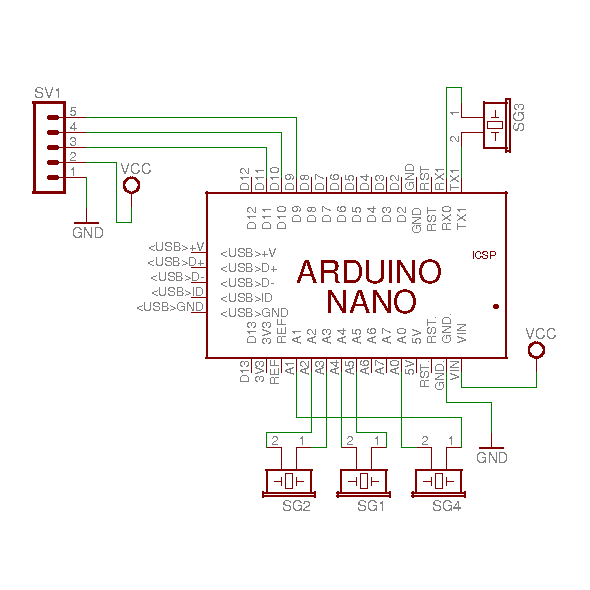
\includegraphics[width=0.6\textwidth, trim= 0mm 0mm 0mm 0mm,clip]{transmitter}
    \caption{Schemat nadajnika}
    \label{fig:nadajnik_schemat}
\end{figure}

Całość umieszczono na ramie w kształcie litery H wykonanej z rurek PCV (rysunek \ref{fig:nadajnik_szkic}).
Rezonatory dodatkowo odizolowano  od ramy przy użyciu rzepów, co ułatwia ich demontaż, a także skutecznie
zapobiega przenoszeniu się drgań. 

\rysunek{nadajnik_H}{Szkic ramy nadajnika}{\label{fig:nadajnik_szkic}}


\textit{Android Nano} połączony jest z odbiornikiem sześciometrowym kablem, którym przesyłane są sygnały sterujące oraz zasilanie.
Do sterowania wykorzystano trzy przewody -- dwa z nich informują, który z głośników ma w danym momencie nadawać,
a trzeci służy jako wyzwalacz. 
Informacja, który z głośników  ma nadawać, kodowana jest za pomocą dwóch bitów w systemie binarnym --
napięcie na przewodzie \SI{3,3}{V} oznacza logiczną jedynkę, a \SI{0}{V} oznacza logiczne zero.

Na potrzeby nadajnika powstało oprogramowanie w C dla procesora ATmega328 generujące nadawany sygnał.
Cała logika programu mieści się w obsłudze przerwania sprzętowego, które reaguje na opadające zbocze na wyzwalaczu.
Gdy następuje przerwanie, oprogramowanie wysyła z góry zdefiniowany sygnał do odpowiedniego rezonatora. 
Nadawany sygnał został tak dobrany, by dało się go w prosty sposób wyodrębnić oraz by trwał jak najkrócej. Składa się z dwóch
części: wzbudzającej i tłumiącej.
Okres impulsów sygnału jest zgodny z częstotliwością rezonansową przetworników, a dodatkowo część tłumiąca
jest przesunięta względem części wyzwalającej o 180 stopni.
Czas trwania części wzbudzającej jest najkrótszy z możliwych i trwa jeden okres, natomiast czas trwania części tłumiącej określono
tak, by odebrany sygnał zawierał również sinusoidy przesunięte fazowo względem początkowej części sygnału.
Rysunek \ref{fig:output_signal} przedstawia sygnał podawany na przetwornik piezoelektryczny.

\begin{figure}[ht]
    \centering
    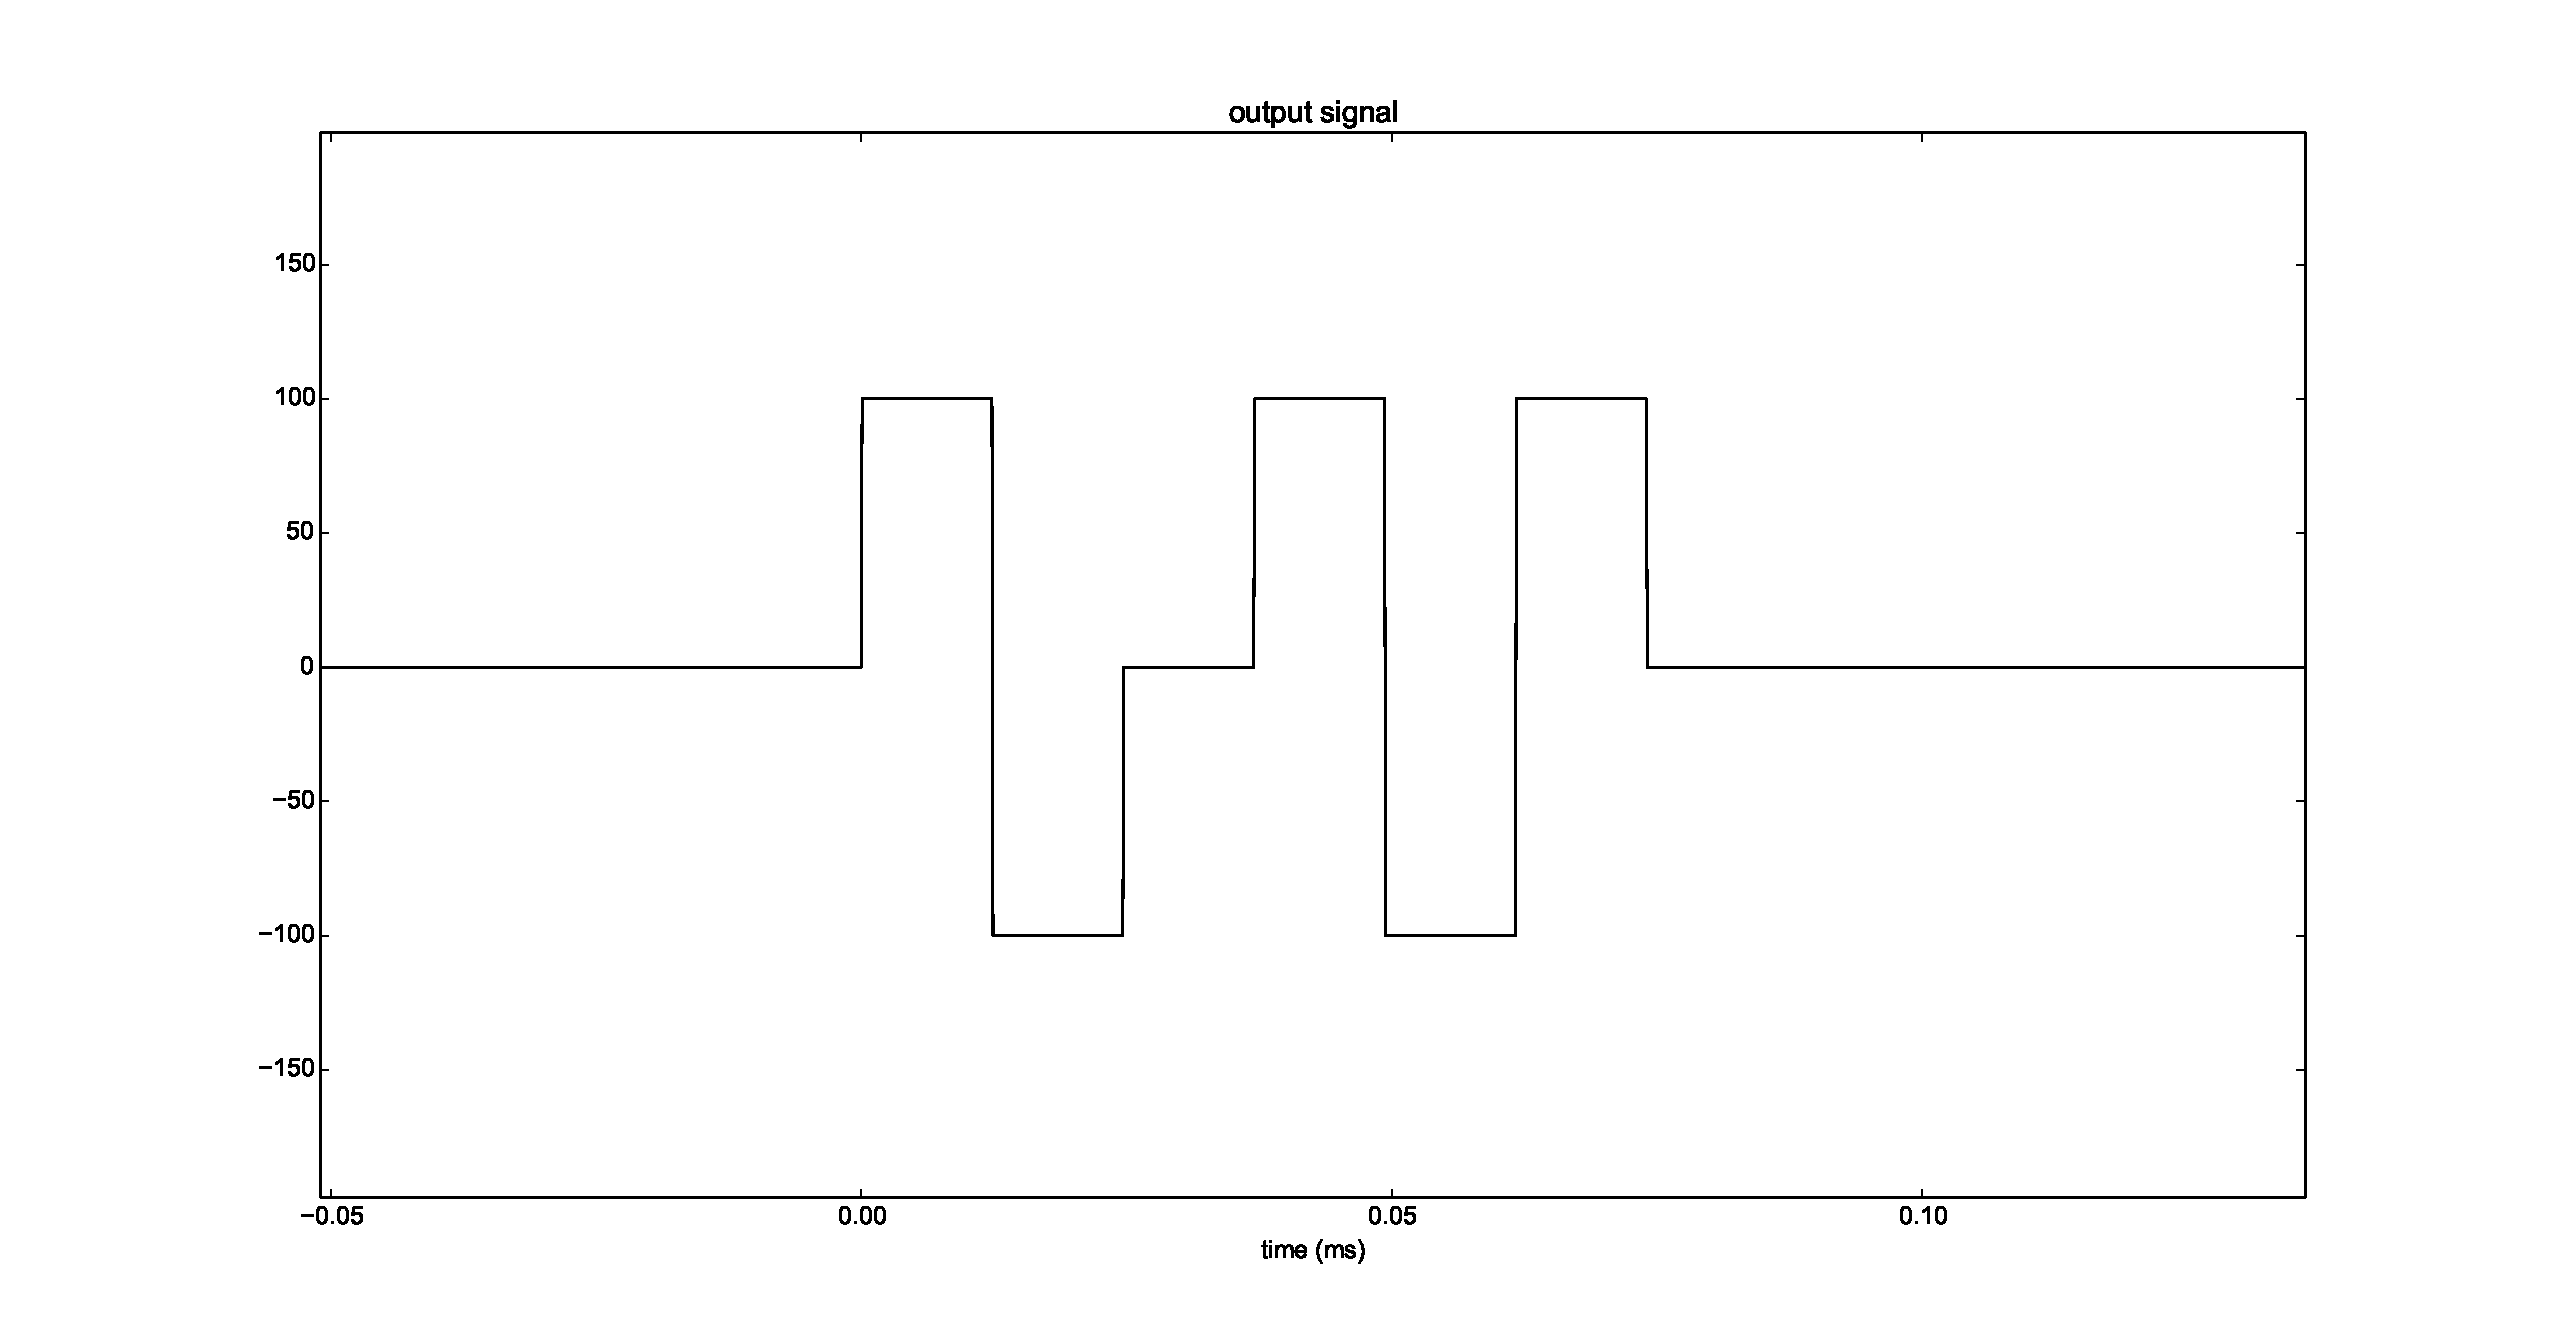
\includegraphics[width=1.0\textwidth, trim= 25mm 0mm 0mm 0mm,clip]{output_signal}
    \caption{Sygnał podawany na przetwornik piezoelektryczny}
    \label{fig:output_signal}
\end{figure}

\section{Dobór rezonatorów piezoelektrycznych}

Głównym problemem podczas konstrukcji nadajnika okazał się dobór odpowiednich rezonatorów piezoelektrycznych.
Mimo że producent wykorzystanych rezonatorów zapewnia ich pracę w zakresie \SI{40}{kHz} $\pm$ \SI{1}{kHz},
to taki rozrzut okazał się zbyt duży, 
dlatego z 30 rezonatorów (15 nadajników i 15 odbiorników) wybrane zostały 4 nadajniki i 3 odbiorniki o najbardziej 
zbliżonych częstotliwościach rezonansowych.
Tabela \ref{table:czestotliwosci} zawiera wyniki pomiarów częstotliwości. Gwiazdką oznaczono wykorzystane przetworniki piezoelektryczne.

\begin{table}[h]
  \caption{Częstotliwości rezonansowe przetworników piezoelektrycznych}
  \smallskip
  \label{table:czestotliwosci}
  \centering
  \begin{tabular}{|r|r|r|}
    \hline 
    Nr & Nadajnik 40ST-12 & Odbiornik 40SR-12\\
    \hline
    1  &   \SI{40,88}{kHz} & *\SI{40,65}{kHz} \\
    2  &   \SI{41,12}{kHz} &  \SI{40,45}{kHz} \\
    3  &  *\SI{40,78}{kHz} &  \SI{39,52}{kHz} \\
    4  &   \SI{41,19}{kHz} &  \SI{40,47}{kHz} \\
    5  &   \SI{40,92}{kHz} &  \SI{40,66}{kHz} \\
    6  &   \SI{39,68}{kHz} & *\SI{40,69}{kHz} \\
    7  &   \SI{39,78}{kHz} &  \SI{40,59}{kHz} \\
    8  &  *\SI{40,80}{kHz} &  \SI{40,39}{kHz} \\
    9  &   \SI{40,90}{kHz} &  \SI{40,29}{kHz} \\
    10 &  *\SI{40,66}{kHz} & *\SI{40,68}{kHz} \\
    11 &  *\SI{40,85}{kHz} &  \SI{39,22}{kHz} \\
    12 &   \SI{41,01}{kHz} &  \SI{39,51}{kHz} \\
    13 &   \SI{41,00}{kHz} &  \SI{39,92}{kHz} \\
    14 &   \SI{39,82}{kHz} &  \SI{39,26}{kHz} \\
    15 &   \SI{39,64}{kHz} &  \SI{39,11}{kHz} \\
    \hline
  \end{tabular}
\end{table}



\section{Odbiornik}

Centralną częścią prezentowanego prototypu stanowi odbiornik.
Jego zadaniem jest wysyłanie sygnałów sterujących do nadajnika, zbieranie ultradźwięków z otoczenia oraz przesyłanie 
ich do komputera w celu dalszej analizy.
Odbiornik składa się z części (rysunek \ref{fig:odbiornik_szkic}):

\begin{itemize}
 \item trzech modułów ultradźwiękowych przetwarzających dźwięk na sygnał elektryczny,
 \item płytki prototypowej \textit{stm32f4-discovery} \cite{bib:stm32f4Discovery} odpowiadającej za komunikację z komputerem,
 \item przystawki do \textit{stm32f4-discovery} przystosowującej sygnały elektryczne z modułów ultradźwiękowych
  do poziomów akceptowalnych przez tę płytkę,
 \item ramy, na której umieszczone są moduły ultradźwiękowe.
\end{itemize}


\rysunek{odbiornik_szkic}{Szkic odbiornika}{\label{fig:odbiornik_szkic}}


\section{Budowa i zasada działania odbiornika}

Głównym elementem odbiornika jest płytka prototypowa \textit{stm32f4-discovery} \cite{bib:stm32f4Discovery}.
 Umożliwia ona komunikację wszystkich komponentów z komputerem.
Oparta jest na procesorze STM32F407VGT6 \cite{bib:stm32f407} typu ARM Cortex M4, 
który zawiera trzy 12-bitowe przetworniki
analogowo-cyfrowe umożliwiające próbkowanie z prędkością do \SI{2,4}{MSPS}. Przetworniki te wykorzystane zostały do próbkowania
sygnałów pochodzących z modułów ultradźwiękowych. Procesor umożliwia również komunikację z komputerem przez 
port USB z prędkością \SI{12}{MB/s}. Na płytce prototypowej znajduje również programator
umożliwiający programowanie procesora i jego testowanie za pośrednictwem dodatkowego portu USB.

Na potrzeby odbiornika powstało dedykowane oprogramowanie w C sterujące procesorem.
Zostało ono oparte na bibliotece \textit{stm32 usb 101} \cite{bib:stm32_usb_101}
zapewniającej komunikację z komputerem, do której dodano obsługę przetworników \textit{ADC}.
Program przez port USB dostaje instrukcję, który z czterech głośników ma nadawać, i przekazuje ją
dalej do nadajnika wraz z sygnałem wyzwalającym. Następnie uruchamiane są równocześnie trzy przetworniki \textit{ADC}, które 
próbkują odbierany dźwięk i poprzez DMA zapisują trzy kanały w pamięci procesora.
Częstotliwość pracy przetworników ustawiono na \SI{1,6}{MSPS}, co daje średnio 40 próbek na jeden okres \SI{40}{kHz} sygnału.
Program zapamiętuje \SI{16}{kS} na każdy kanał, co przy prędkości dźwięku \SI{340}{m/s} pozwala zmierzyć odległość
wynoszącą maksymalnie 2,5 metra.

Po zebraniu w sumie \SI{48}{kS}, całość przesyłana jest do komputera w celu dalszej analizy.
Proces powtarzany jest dla każdego z czterech głośników nadajnika, 
co w sumie daje 12 sygnałów, na podstawie których wyznaczona zostaje 
pozycja w przestrzeni oraz orientacja nadajnika.

Cała elektronika osadzona została na ramie w kształcie trójkąta zbudowanej z rur PCV  (rysunek \ref{fig:trojkat}). 
Odległości pomiędzy modułami ultradźwiękowymi są z góry ustalone, co ułatwia dalsze obliczenia.

\rysunek{trojkat}{Szkic ramy odbiornika}{\label{fig:trojkat}}



\clearpage
\section{Budowa modułu ultradźwiękowego}

Odbiornik wyposażony został w trzy moduły ultradźwiękowe, których zadaniem jest 
zbieranie ultradźwięków z trzech różnych  punktów.
Każdy z modułów zawiera przetwornik piezoelektryczny (mikrofon) 40SR-12 \cite{bib:40ST12},
który przetwarza sygnał akustyczny na odpowiadający mu sygnał elektryczny, oraz wzmacniacze operacyjne 
wstępnie zwiększające amplitudę sygnału, który przesyłany jest dalej do przystawki.
Rysunek \ref{fig:odbiornik_ultra} przedstawia schemat modułu ultradźwiękowego.

\rysunek{receiver}{Schemat modułu ultradźwiękowego}{\label{fig:odbiornik_ultra}}

Wzmacniacz operacyjny IC1A wraz z kondensatorem C2 i rezystorem R1 pracuje 
jako przedwzmacniacz ładunkowy \cite{bib:wzm_ladunkowy}.
Ładunek wytworzony na przetworniku piezoelektrycznym SP1 zostaje w całości przeniesiony na kondensator C2 
(wzmacniacz utrzymuje różnicę potencjałów między dodatnim a ujemnym wejściem na zerowym poziomie).
W wyniku czego na kondensatorze pojawia się napięcie zgodnie z równaniem $U=\frac{q}{C}$.
Zadaniem rezystora R1 jest rozładowanie kondensatora C2,
R1 i C2 działają również jako filtr dolnoprzepustowy.
Wzmacniacz IC1B z rezystorami R5 i R4 oraz kondensatorami C3, C7 i C8 pracuje jako wzmacniacz napięciowy wzbogacony o 
filtr pasmowoprzepustowy.
W celu zminimalizowania zakłóceń zastosowano niskoszumowe wzmacniacze operacyjne
mieszczące się w jednym układzie scalonym NE5532 \cite{bib:ne5532}, 
dodatkowo płytka drukowana jest ekranowana.

Wzmocniony sygnał doprowadzony jest przez wtyczkę JP1 do przystawki współpracującej z \textit{stm32f4-discovery}.

\section{Przystawka do \textit{stm32f4-discovery}}

Sygnał z modułów ultradźwiękowych dociera do \textit{stm32f4-discovery} za pośrednictwem specjalnej przystawki.
Schemat budowy przystawki przedstawia rysunek \ref{fig:przystawka}.
Zadaniem przystawki jest przystosowanie maksymalnych amplitud zebranych sygnałów do wartości akceptowalnych przez  
przetworniki analogowo-cyfrowe procesora STM32F407VGT6.
Wartości te muszą mieścić się w zakresie od \SI{0}{V} do \SI{3,3}{V}.

Zastosowano w niej układ TLV2774 \cite{bib:TLV2774}, który zawiera 4 wzmacniacze operacyjne typu
\textit{rail-to-rail}. Trzy z nich wykorzystano jako ostatni stopień wzmocnienia sygnałów ultradźwiękowych. 
Wzmacniacze operacyjne pracują w układzie odwracającym, którego wzmocnienie można regulować potencjometrami R8, R9, R10. 
Podłączono je do wspólnego, również regulowanego (potencjometr R7) napięcia odniesienia.
Przystawka zawiera także stabilizator napięcia LM78M05CDT \cite{bib:LM78M05CDT}, który po podłączeniu 
do JP4 baterii \SI{12}{V} dostarcza zasilanie do wszystkich komponentów. 
Istnieje możliwość odcięcia zasilania poprzez rozwarcie JP5, co jest konieczne podczas programowania
STM32F407VGT6 by nie uszkodzić stabilizatora napięcia.
Z przystawki przez wtyczkę JP6 wyprowadzono również sygnały sterujące nadajnikiem oraz zasilanie.

 \begin{figure}[h!]
    \centering
    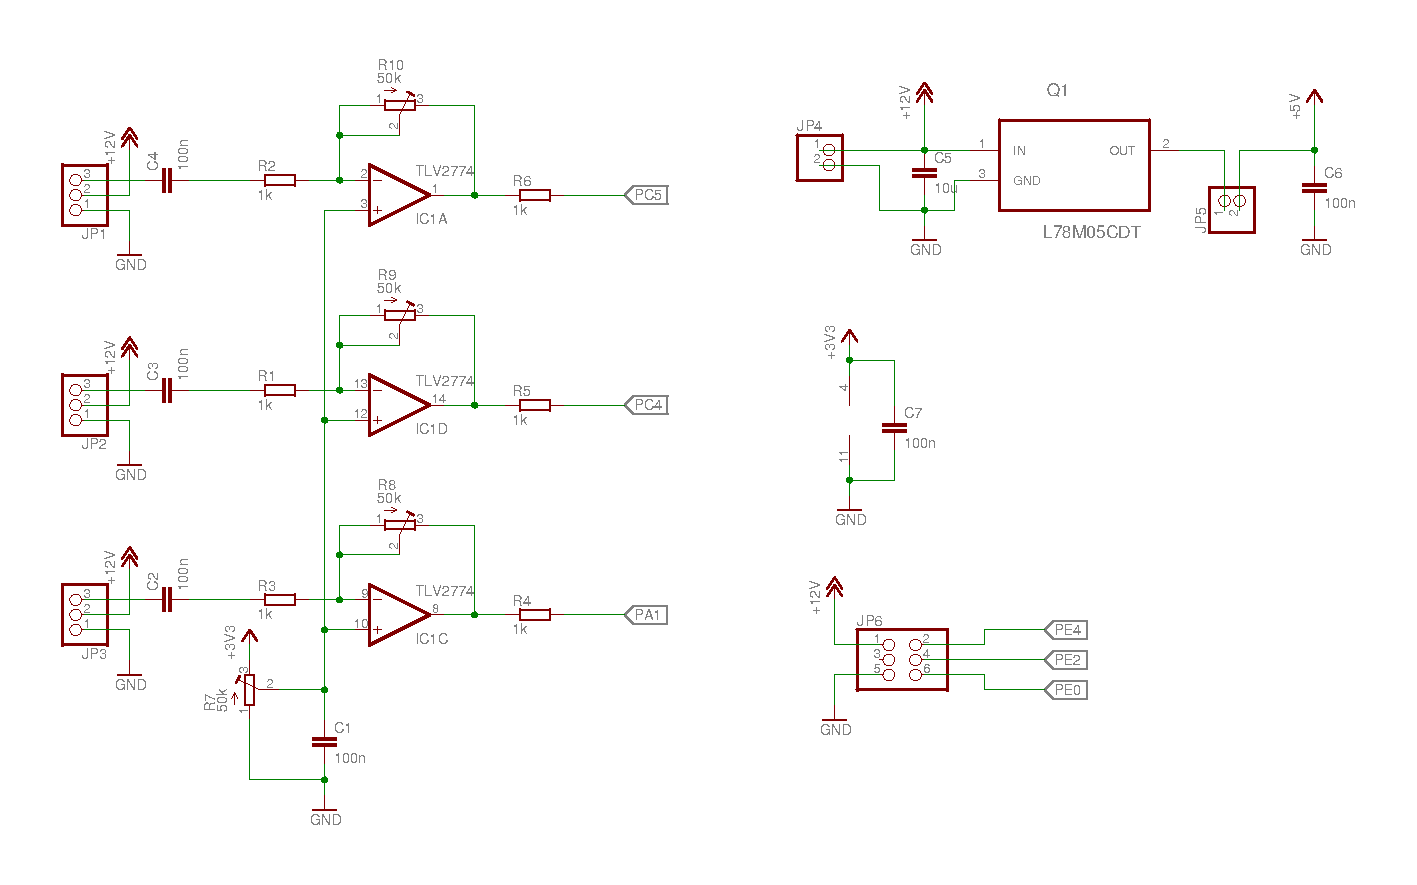
\includegraphics[width=1\textwidth, trim= 5mm 0mm 0mm 0mm,clip]{mainboard2}
    \caption{Schemat budowy przystawki do \textit{stm32f4-discovery}}
    \label{fig:przystawka}
\end{figure}



\chapter{Przetwarzanie danych zebranych z odbiorników}

Najważniejszą częścią prototypu jest oprogramowanie, które przekształca surowe dane dźwiękowe
z odbiornika na położenie nadajnika w przestrzeni oraz jego orientację.

Przetwarzaniem danych zajmuje się biblioteka \textit{mp3d}
oraz program \textit{scan.py} wizualizujący dane w postaci obrazu trójwymiarowego.

Biblioteka \textit{mp3d} została podzielona na pięć modułów:
\begin{enumerate}

 \item \textit{com.py} - moduł odpowiedzialny za komunikację odbiornikiem
 \item \textit{find\_pattern.py} - moduł odpowiedzialny za wyszukanie wzorca w odebranym sygnale
 \item \textit{xyz.py} - moduł odpowiedzialny za wyznaczenie pozycji i orientacji nadajnika, oraz za 
 weryfikację, czy zebrane dane odpowiadają rzeczywistości
 \item \textit{info.py} - moduł wyświetlający informację o sile odbieranego sygnału
 \item \textit{ply.py} - moduł odpowiedzialny za eksportowanie danych do formaty \textit{.ply} 
    (Polygon File Format) obsługiwanego przez większość programów do obróbki grafiki 3D.

\end{enumerate}


\section{Moduł \textit{com.py}}

Zadaniem modułu \textit{com.py} jest komunikacja poprzez port USB odbiornikiem,
moduł pracuje w oddzielnym wątku, w którym cyklicznie wysyła żądanie by dany głośnik nadał sygnał, następnie odbiera
sygnał z trzech mikrofonów.
Ta czynność powtarzana jest dla każdego z czterech nadajników. 
Zebrane dwanaście sygnałów po wstępnej filtracji przekazywane są dalej do \textit{find\_pattern.py}. Cały cykl powtarzany jest
co 200ms. Rysunek \ref{fig:com_output_2m} przedstawia sygnał z jednego mikrofonu przekazywany do modułu \textit{find\_pattern.py}.


\begin{figure}[h!]
    \centering
    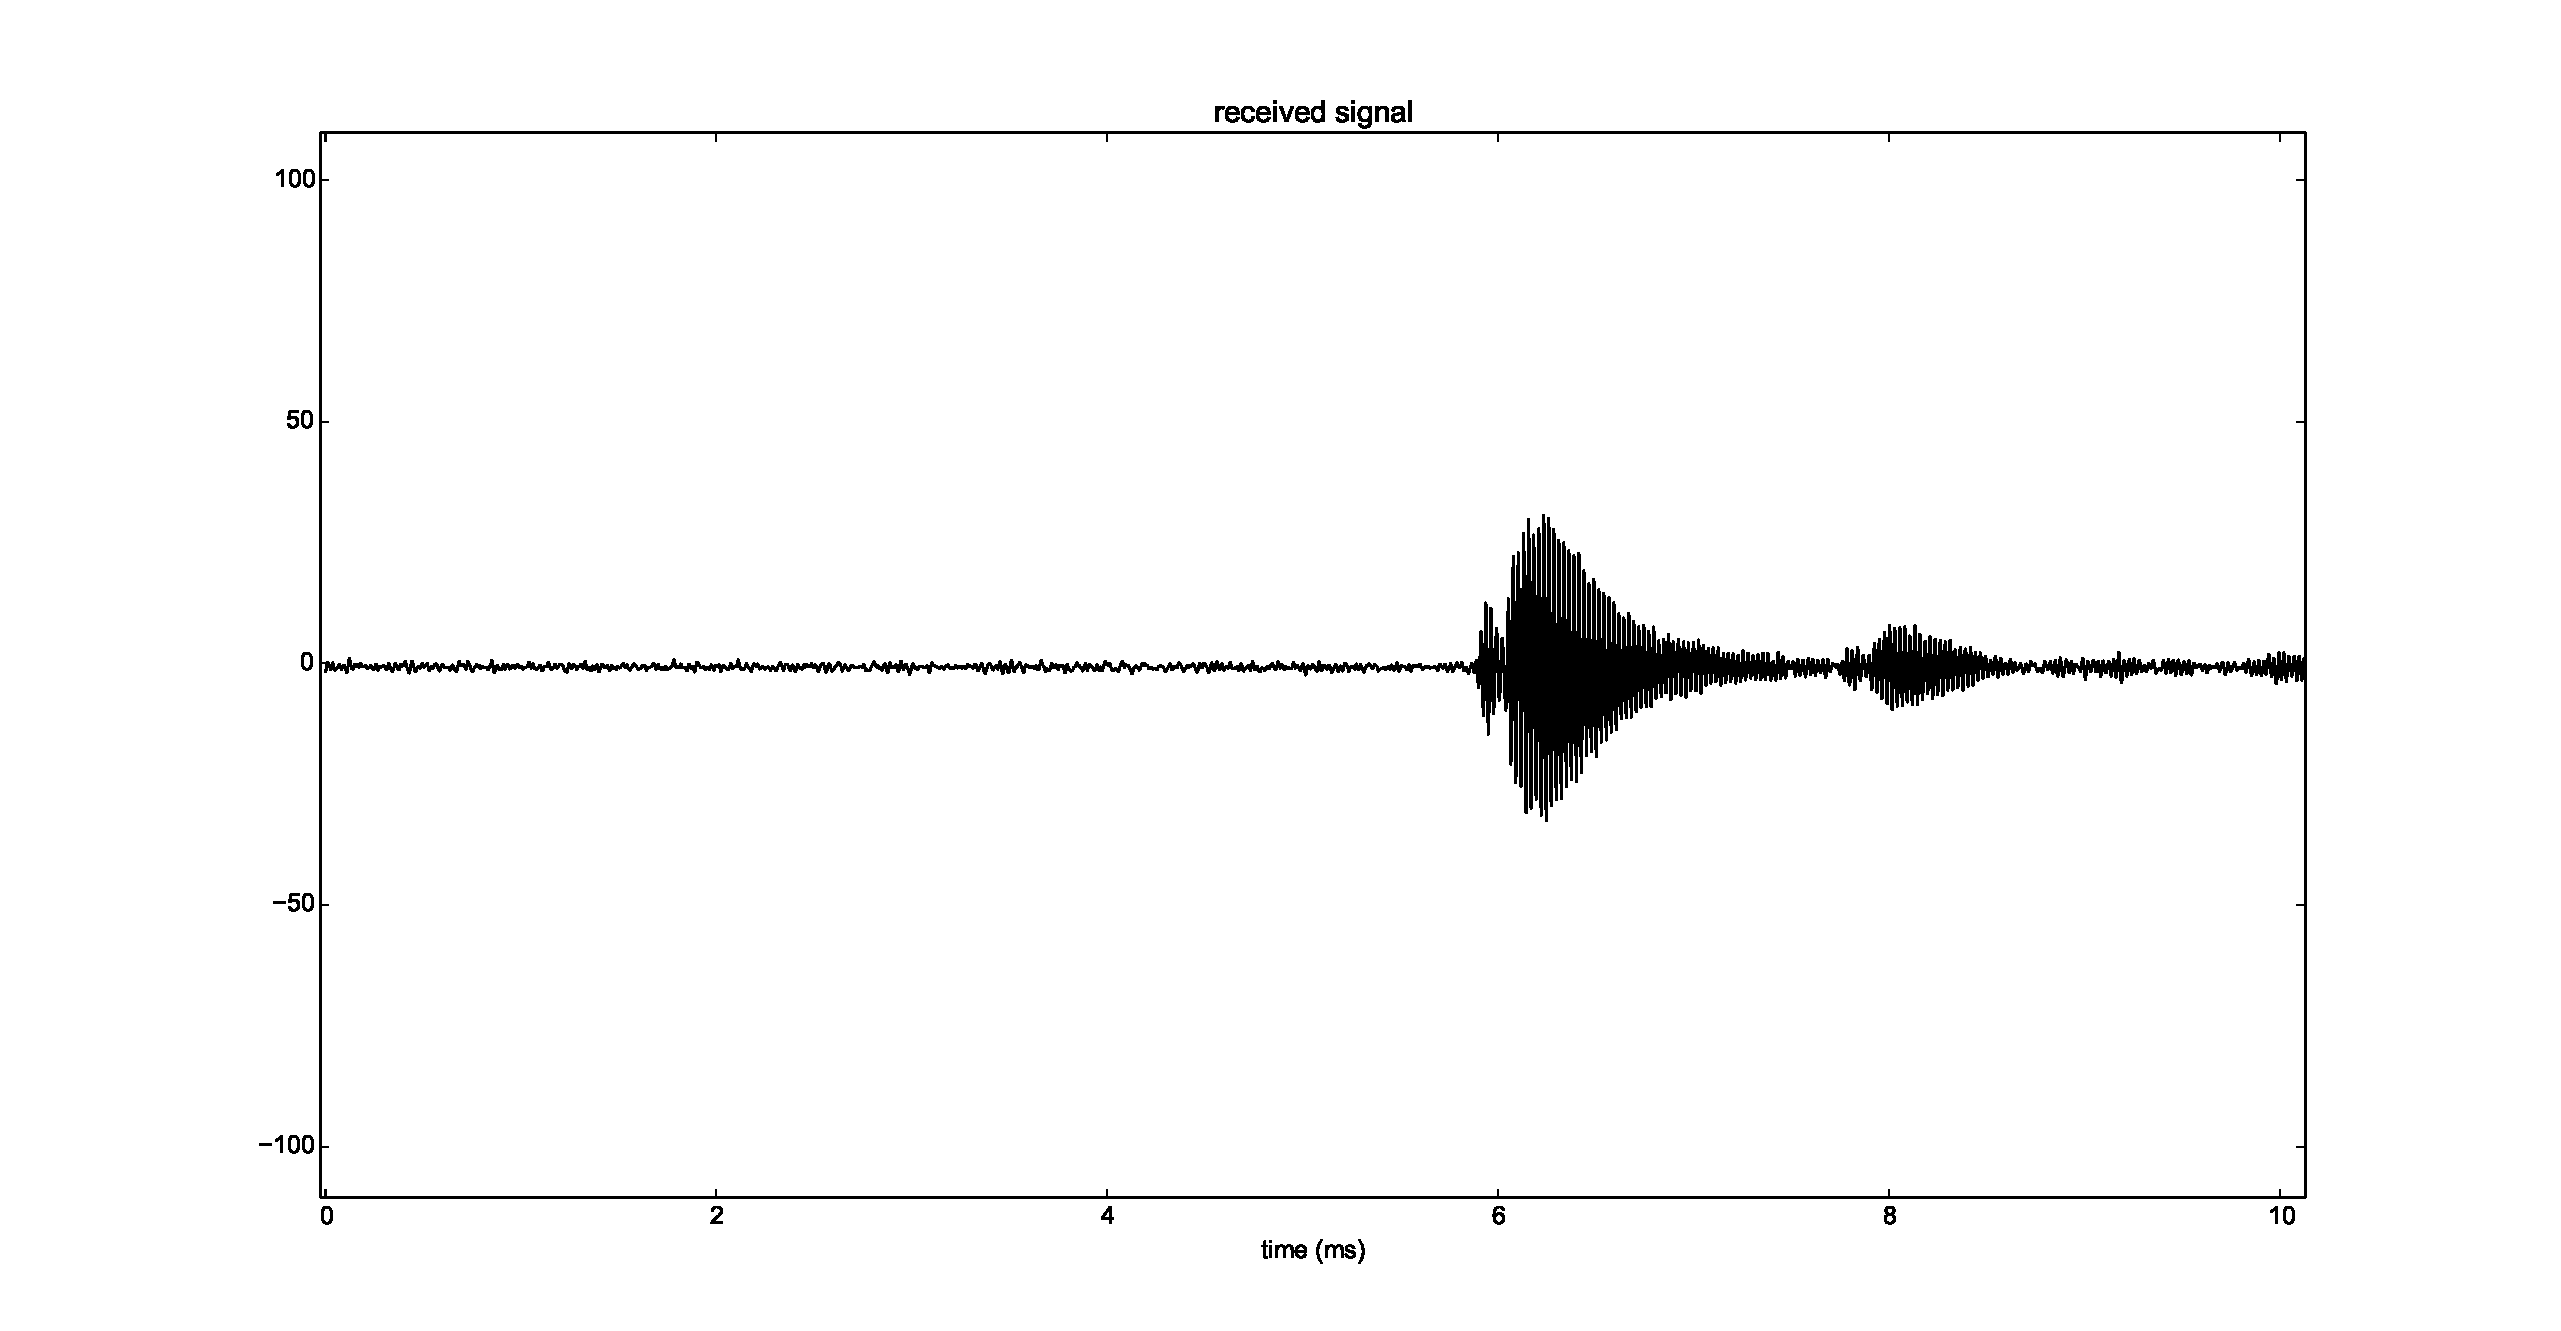
\includegraphics[width=1.15\textwidth, trim= 47mm 0mm 0mm 0mm,clip]{com_output_2m_1}
    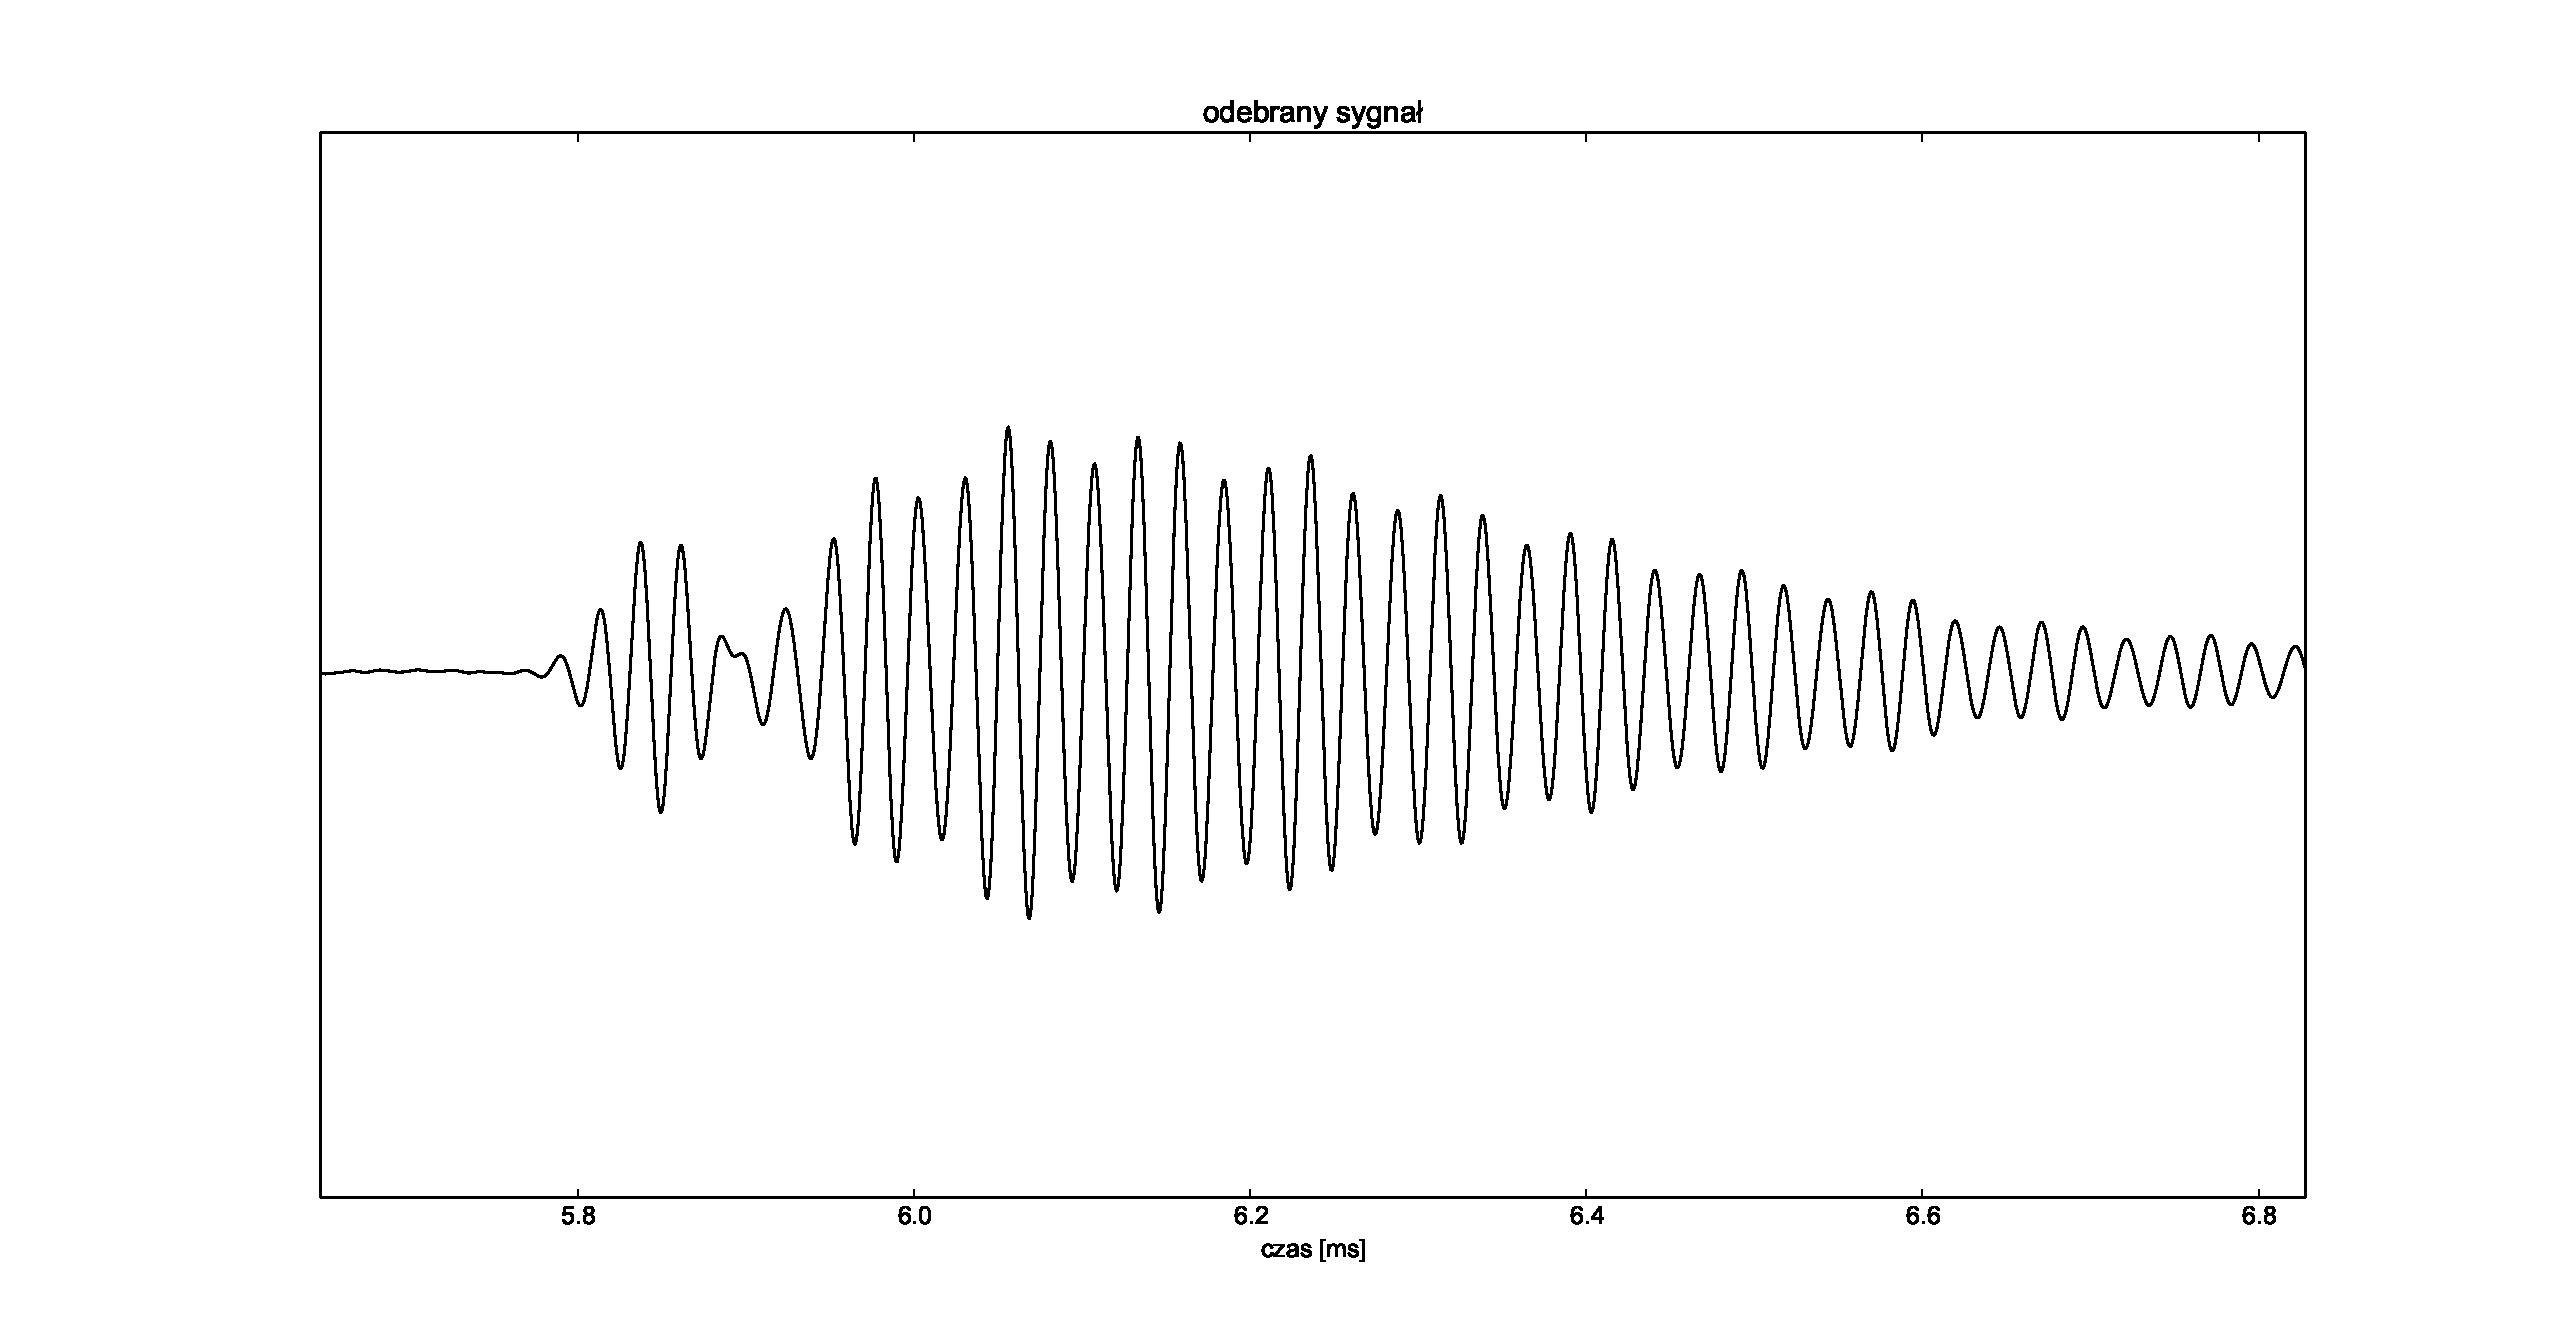
\includegraphics[width=1.15\textwidth, trim= 47mm 0mm 0mm 0mm,clip]{com_output_2m_2}
    \caption{sygnał odebrany przez moduł \textit{com.py}. 
    Odległość między nadajnikiem a odbiornikiem wynosi 2 metry.
    Na górnym wykresie po prawej stronie widoczne są również sygnały odbite od ścian.
    }
    \label{fig:com_output_2m}
\end{figure}


\section{Moduł \textit{find\_pattern.py}}

Głównym modułem biblioteki \textit{mp3d} jest moduł \textit{find\_pattern.py}.
Odpowiada on za znalezienie \textit{wzorca} w odebranym sygnale.
Odbierane sygnały zmieniają się nieznacznie podczas pracy skanera (głównie gdy kąt nachylenia nadajnika względem odbiornika się zmienia)
dlatego wzorzec początkowo wprowadzony jest podczas kalibracji następnie jest ciągle aktualizowany jeśli odebrany sygnał ma wystarczającą moc.
Do wyszukania wzorca wewnątrz sygnału wykorzystana jest metoda najmniejszego błędu średniokwadratowego.

Niech $w(t)$  dla $t = 0..n-1$ będzie szukanym wzorcem, a $f(x)$ odebranym sygnałem,
wtedy możemy znaleźć takie $a$, że błąd średniokwadratowy pomiędzy $w(t)$ i $a f(t+x)$ jest minimalny, mianowicie:
\[
  E(x) = \min_{a \in R} \{ \sum_{t=0}^{n-1}  (w(t) - a f(t+x))^2 \}
\]
gdzie $E(x)$ jest bezwzględnym błędem średniokwadratowym, zauważmy że:
\[
  E(x) = \min_{a \in R} \{ \sum_{t=0}^{n-1}  (w^2(t) -2a w(t) f(t+x) + a^2 f^2(t+x)) \}
\]
\[
  E(x) = \min_{a \in R} \{ \sum_{t=0}^{n-1}  w^2(t) -2a \sum_{t=0}^{n-1}  w(t) f(t+x) + a^2 \sum_{t=0}^{n-1} f^2(t+x) \}
\]
funkcja kwadratowa w postaci:
\[
  y(a) = \sum_{t=0}^{n-1}  w^2(t) -2a \sum_{t=0}^{n-1}  w(t) f(t+x) + a^2 \sum_{t=0}^{n-1} f^2(t+x)
\]
osiąga minimum dla:
\[
 a = \frac{ \sum\limits_{t=0}^{n-1}  w(t) f(t+x) }{ \sum\limits_{t=0}^{n-1} f^2(t+x) }
\]
z czego ostatecznie dostajemy:

\[
  E(x) = \sum_{t=0}^{n-1}  w^2(t)  - \frac {(\sum\limits_{t=0}^{n-1}  w(t) f(t+x) )^2 } { \sum\limits_{t=0}^{n-1} f^2(t+x)}
\]

Zauważmy, że dzięki skalowaniu sygnału $f(x)$ zamiast sygnał wzorcowy $w(x)$
otrzymany błąd $E(x)$ nie zależy od siły odebranego sygnału, co ułatwia porównanie błędów w dwóch różnych miejscach,
Zależy on jednak od siły sygnału wzorcowego, aby się od niego uniezależnić możemy wyznaczyć
błąd względny:
\[
  e(x) = \frac{E(x)}{\sum\limits_{t=0}^{n-1}  w^2(t)}
\]

\[
  e(x) = 1 - \frac {(\sum\limits_{t=0}^{n-1}  w(t) f(t+x) )^2 } { \sum\limits_{t=0}^{n-1} f^2(t+x) \sum\limits_{t=0}^{n-1}  w^2(t)}
\]

Ponadto wyliczenie $ \sum\limits_{t=0}^{n-1}  w^2(t) $ 
jak i $\sum\limits_{t=0}^{n-1} f^2(t+x)$ wymaga jedynie liniowej liczby operacji, a 
 $\sum\limits_{t=0}^{n-1}  w(t) f(t+x)  $ jest korelacją wzajemną funkcji $w(t)$ i $f(x)$, którą
 można wyliczyć w czasie $n \log(n)$ korzystając z szybkiej transformacji Fouriera \cite{bib:FFT_correlation}.
 
 Funkcję $e(x)$  można ją interpretować jako:
 im mniejszy błąd $e(x)$ tym większe prawdopodobieństwo, że szukany wzorzec $w$ znajduje się na pozycji $x$ w 
 odebranym sygnale $f$. 
 Wynikiem modułu \textit{find\_pattern.py} jest cała funkcja, $e(x)$ na podstawie której moduł \textit{xyz.py}
 wyznaczy pozycję głowicy w przestrzeni jak i jego orientację uwzględniając przy tym 
 kształt głowicy (nadmiarowość danych) jak i prawdopodobieństwa że znaleziony wzorzec jest na danej pozycji.
 
 Kolejną zadaniem modułu \textit{find\_pattern.py} jest uaktualnianie wzorca z biegiem czasu.
 Wraz ze zmianą kąta nachylenia nadajnika względem odbiornika zmienia się znacząco kształt odbieranego sygnału,
 dlatego jeśli odnajdziemy szukany wzorzec, którego moc sygnału jest wystarczająco silna to
 podmieniany jest na niego wzorzec.
 
 Na rysunku \ref{fig:blad_korel} przedstawiony jest wynik przetwarzania sygnału przez moduł \textit{find\_pattern.py}.
 
 \begin{figure}[h!]
    \centering
    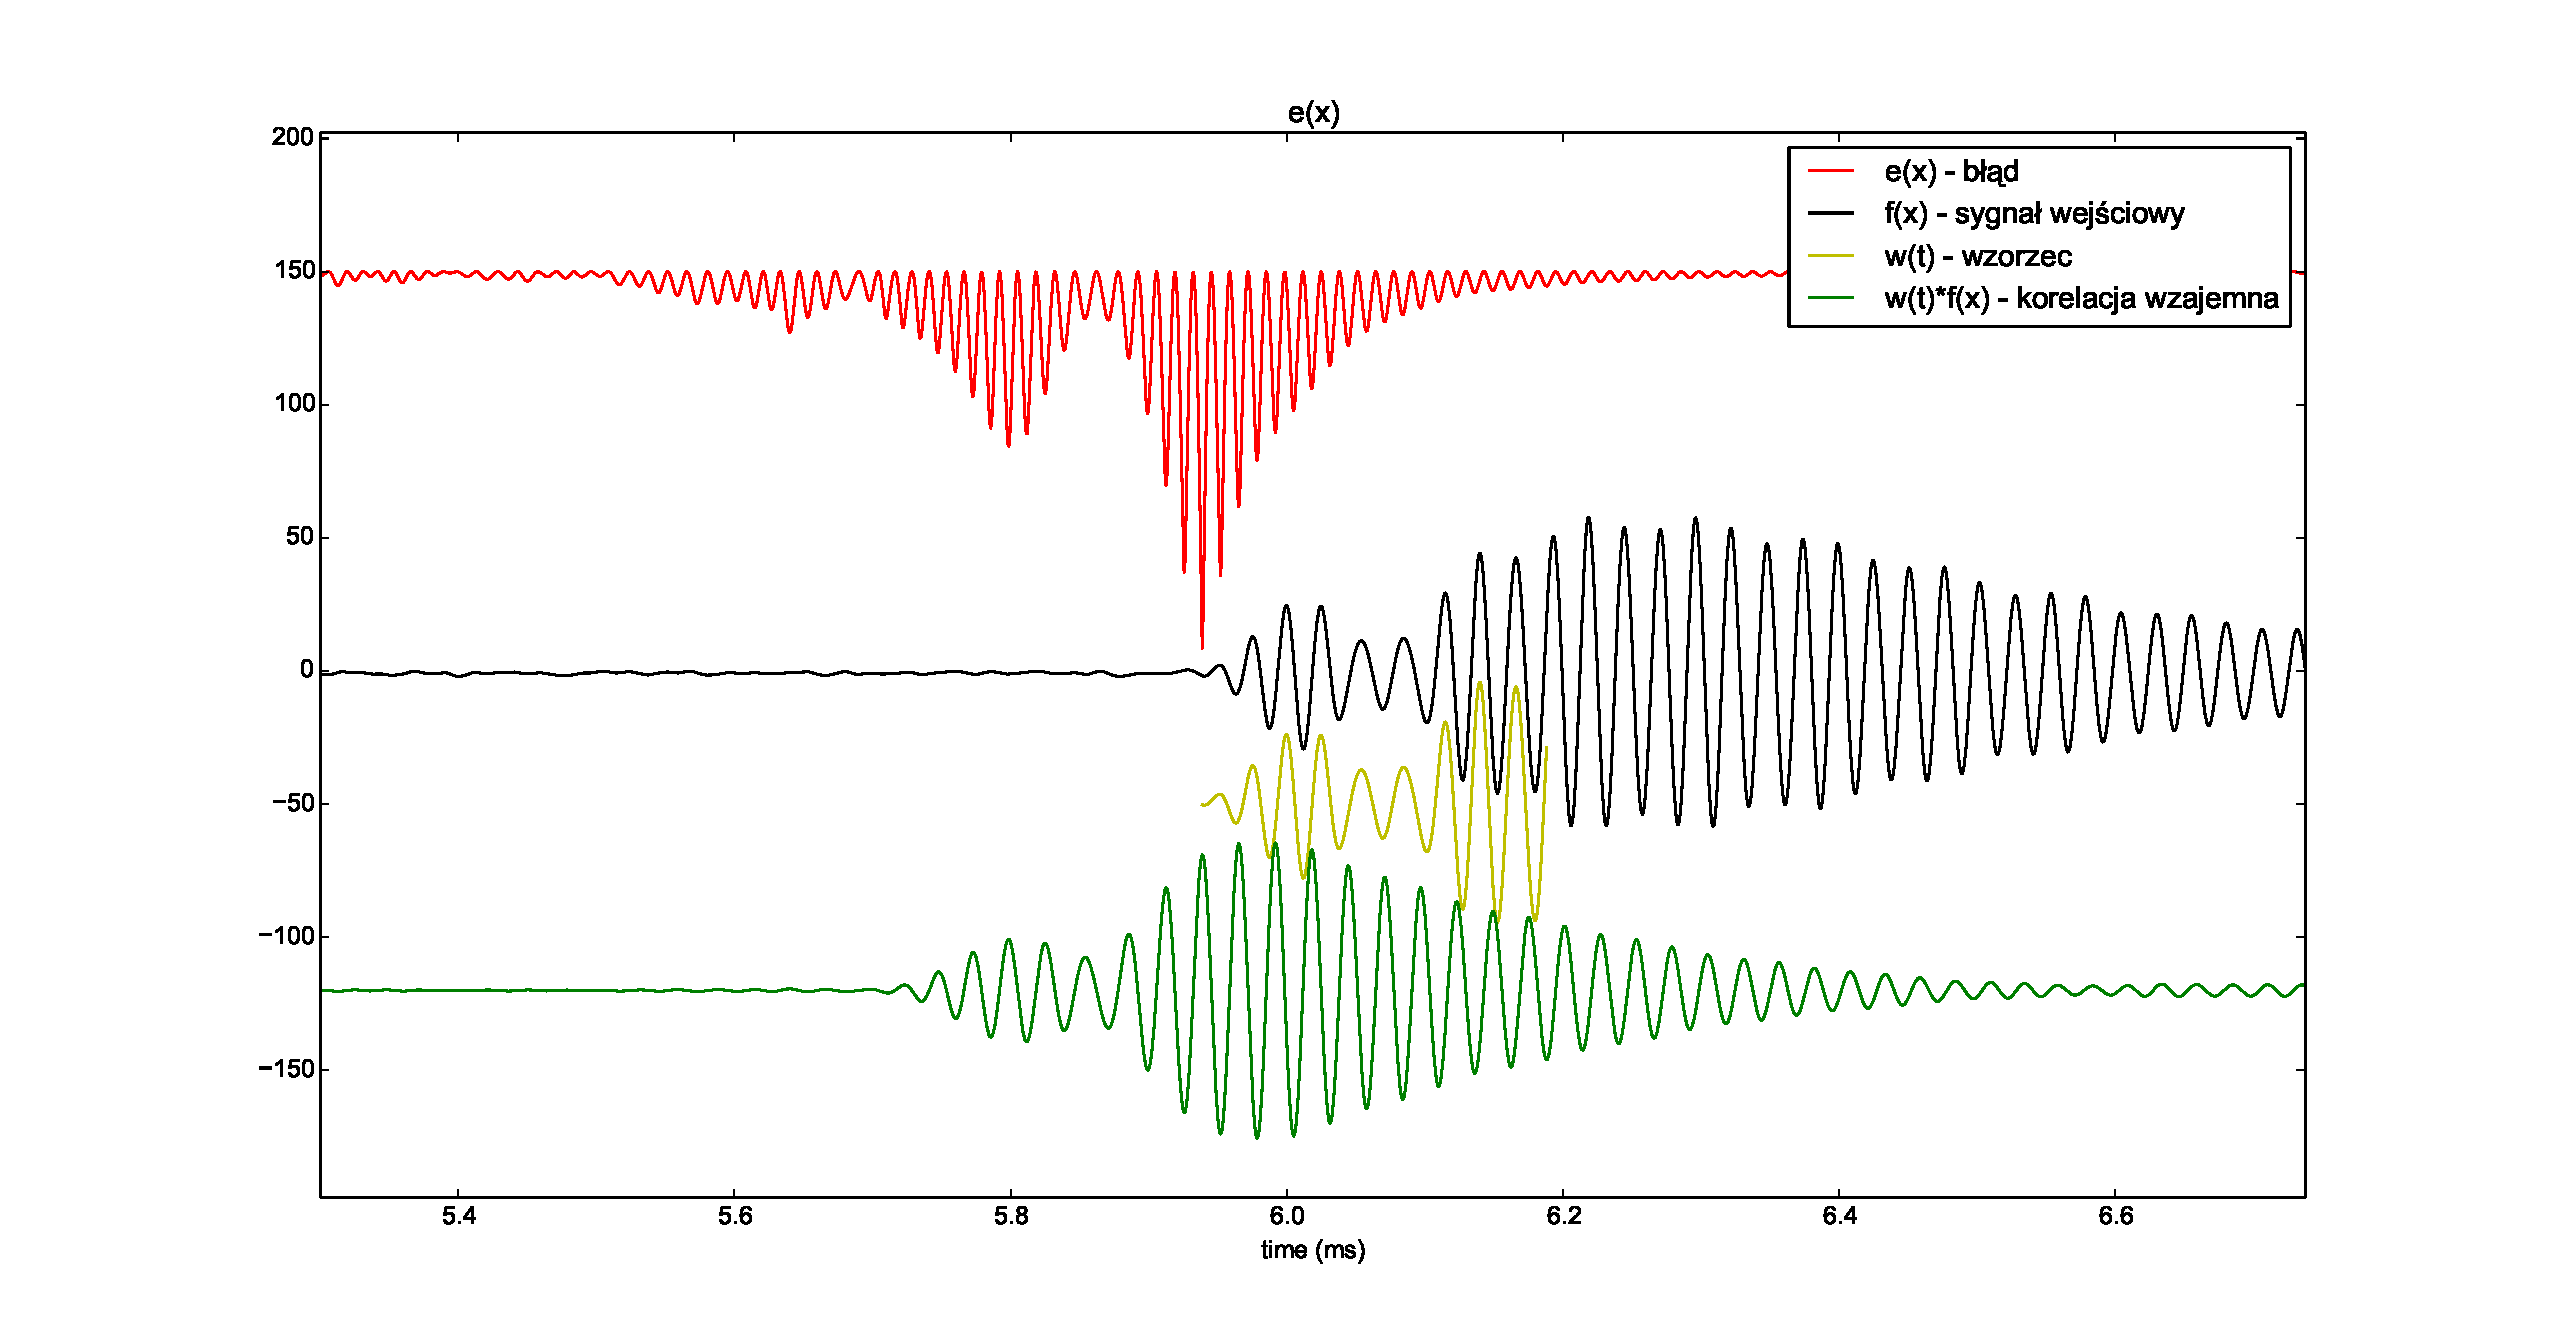
\includegraphics[width=1.15\textwidth, trim= 47mm 0mm 0mm 0mm,clip]{blad_korel}
    \caption{sygnał przetworzony przez moduł \textit{find\_pattern.py}.}
    \label{fig:blad_korel}
\end{figure}
 

 
\section{Moduł \textit{xyz.py}}

Zadaniem modułu \textit{xyz.py} jest wyznaczenie pozycji oraz orientacji w przestrzeni głowicy nadajnika.
Zauważymy, że moduł musi wyznaczyć trzy współrzędne $(x_1,x_2,x_3)$
oraz trzy kąty nachylenia $(\alpha_1, \alpha_2, \alpha_3)$ czyli w sumie sześć niewiadomych.
Na wejściu moduł pobiera dwanaście sygnałów $e_i(x)$ dla $i=0..11$ odpowiadających prawdopodobieństwom odległości
czterech nadajników od trzech odbiorników, mamy więc dwukrotną nadmiarowość danych.
Ta nadmiarowość wykorzystywana jest do korekcji błędów podczas pomiaru odległości.
Moduł wybiera $n$ najbardziej prawdopodobnych odległości z $e_i(x)$, czyli takich $x_ij$ dla $j = 0...n-1$
że $e_i(x_ij)$ jest duże, następnie sprawdza która kombinacja 
odległości jest możliwa ze względu na poprzedni pomiar (czy głowica nie przemieściła się za szybko)
oraz ze względu na kształt samej głowicy - jeśli wyznaczony kształt głowicy nie pasuje do jej rzeczywistych
rozmiarów pomiar jest odrzucany.
Tak wyznaczone $x_ij$ są przekazywany z powrotem do modułu \textit{find\_pattern.py} w celu odświeżenia wzorca,
oraz na ich podstawie wyznaczana jest pozycja i orientacja głowicy.

\section{Moduł \textit{info.py}}

zadaniem modułu \textit{info.py} jest wyświetlenie informacji związanych z siłą odbieranych sygnałów.

\section{Kalibracja}

Przed każdym uruchomieniem urządzenia wymagana jest kalibracja.
Kalibracja sprowadza się do ustawienia głowicy w odległości 2 metrów od odbiornika
uruchomienia urządzenia oraz zaznaczenia 12 wzorców potrzebnych do odnalezienia 
odebranego sygnału.
Program na podstawie odległości i czasu dodarcia sygnału wylicza prędkość dźwięku 
w danym środowisku. Co ciekawe, wypadkową wyliczonej prędkości jest temperatura otoczenia.

Rysunek \ref{fig:blad_korel} przedstawia widok 12 sygnałów wraz z zaznaczonymi wzorcami.





%\chapter{Kalibracja}\label{r:kalibracja}

Do poprawnego działania prototupu niezbędne są wzorce 
\chapter{Podsumowanie}

W niniejszej pracy przedstawiono urządzenie, które za pomocą ultradźwięków  potrafi określić zarówno swoje
położenie, jak i orientację w przestrzeni.

Mimo że przy pomiarze położenia wykorzystywane są fale dźwiękowe o długość \SI{8}{mm}, urządzenie to
potrafi osiągnąć rozdzielczość  rzędu \SI{0,5}{mm}, co znacząco wyróżnia je na tle innych rozwiązań.
Posiada także inne zalety, jak również wady, które opisano poniżej.
\newline
Zalety:
\begin{itemize}
 \item Wysoka rozdzielczość pomiaru. Zastosowanie częstotliwości 
 próbkowania dużo wyższych od częstotliwości nadawanego sygnału, a także wyszukiwanie wzorca pozwoliły
 wielokrotnie zwiększyć rozdzielczość pomiaru w stosunku do długości wykorzystanej fali dźwiękowej.
 
 \item Praktycznie nieograniczona przestrzeń robocza. Mimo że w prezentowanym prototypie
 ograniczono przestrzeń roboczą do sześcianu \SI{2,5}{m} $\times$ \SI{2,5}{m} $\times$ \SI{2,5}{m},
 jest to jedynie ograniczenie praktyczne i bez trudu można dowolnie zwiększyć tę przestrzeń. Trzeba jednak 
 pamiętać, że siła sygnału dźwiękowego maleje kwadratowo wraz z odległością, więc przy dużo większych odległościach
 niezbędne staje się zastosowanie nadajników większej mocy. 
 
 \item Niski koszt komponentów.
\end{itemize}

Wady:
\begin{itemize}
 \item Duża czułość na zmiany temperatury. Jest to najpoważniejsza wada prezentowanego rozwiązania.
 Zauważmy, że zmiana temperatury otoczenia o $ 1\arcdeg\ $ powoduje zmianę prędkości dźwięku o 0,17\%,
 co przy rozdzielczości \SI{5000}{px} w skrajnych przypadkach daje przesunięcie \SI{7.5}{px}.
 Co prawda w warunkach laboratoryjnych nie stanowi to większego problemu, jednak w praktycznych zastosowaniach
 jest poważnym ograniczeniem.
 
 \item Długi czas odświeżania. Prezentowany prototyp dokonuje pomiarów co \SI{350}{ms}, czyli około 3 pomiarów 
 na sekundę. Ponieważ mierzymy cztery niezależne sygnały (z czterech głośników), poszczególne sygnały mierzone są co \SI{87}{ms}.
  Dźwięk poruszający się z prędkością \SI{346}{m/s}  przebędzie  w tym czasie odległość \SI{29.7}{m}.
 Tak duży dystans w stosunku do powierzchni roboczej jest konieczny, by zapobiec nakładaniu się sygnałów
 (które po odbiciu się od ścian mogłyby wpłynąć na kolejne pomiary; czas rzędu \SI{87}{ms} pozwala 
 na ich całkowite rozproszenie).
 Zakłócaniu pomiarów można także zaradzić, nadając za każdym razem inny rozróżnialny sygnał, to podejście 
 wymaga jednak nadajników i odbiorników o większych możliwościach wysterowania.
 
 \item Stosunkowo mały kąt widzenia. Zastosowane przetworniki piezoelektryczne są przetwornikami kierunkowymi, co 
 ogranicza  maksymalny kąt, pod jakim można ustawić nadajnik względem odbiornika. W prezentowanym 
 prototypie kąt ten nie powinien przekraczać \ang{45}. Zastosowanie większej liczby przetworników lub innego ich rodzaju
 pozwoliłoby znacznie zwiększyć te kąt.

 \item Ograniczone możliwości wysterowania rezonatorów piezoelektrycznych. 
 Zastosowane rezonatory nie nadają się do generowania krótkich impulsów, co zdecydowanie uprościłoby mierzenie odległości.
 
 \item Problem z ustaleniem pozycji i orientacji nadajnika w ruchu. W prezentowanym urządzeniu 
 jeden pomiar pozycji i orientacji wymaga pomiaru położenia czterech głośników w różnych odstępach czasu.
 Jeśli podczas takiego pomiaru nadajnik porusza się ze zbyt dużą prędkością, to otrzymamy położenie
 przesunięte względem siebie zgodnie z kierunkiem ruchu nadajnika. Takie przesunięcie negatywnie wpływa na 
 pomiar orientacji. 
\end{itemize}


Reasumując, prezentowane urządzenie, wykorzystujące ultradźwięki do określania pozycji i orientacji,
jest innowacyjną propozycją, która zapewnia znacznie większą dokładność niż wszystkie inne dostępne rozwiązania.
Najistotniejszą jego wadą wydaje się jednak duża wrażliwość na warunki atmosferyczne, a szczególnie zmianę temperatury.
Jest to zapewne główny powód, dlaczego rozwiązanie to nie znajdzie  szerokiego zastosowania w produktach komercyjnych.




\appendix
\chapter{Załączniki}

Na płycie CD-ROM dołączonej do niniejszej pracy znajdują się:
\begin{itemize}
 \item kopia niniejszej pracy w PDF i jej tekst źródłowy w języku \LaTeX,
 \item kod źródłowy nadajnika,
 \item kod źródłowy odbiornika,
 \item kod źródłowy programu \textit{scan.py} 
 \item kod źródłowy programu do kalibracji \textit{save-pattern.py}
 \item kod źródłowy biblioteki \textit{mp3d}, na którą składają się:
  \begin{itemize}
    \item moduł \textit{mp3d/com.py}
    \item moduł \textit{mp3d/find\_pattern.py}
    \item moduł \textit{mp3d/info.py}
    \item moduł \textit{mp3d/ply.py}
    \item moduł \textit{mp3d/xyz.py}
  \end{itemize} 
\end{itemize}


\begin{thebibliography}{99}

\addcontentsline{toc}{chapter}{Bibliografia}

  \bibitem{bib:soundSpeed}  Dean, E. A., \textit{Atmospheric Effects on the Speed of Sound}, BATTELLE COLUMBUS LABS DURHAM NC, AUG 1979
  \myurl{http://www.dtic.mil/cgi-bin/GetTRDoc?Location=U2&doc=GetTRDoc.pdf&AD=ADA076060}

  \bibitem{bib:stm32_usb_101} Marcin Peczarski, 
  \textit{USB dla niewtajemniczonych w przykładach na mikrokontrolery STM32}, Wydawnictwo BTC, Legionowo 2013,
  \myurl{http://www.mimuw.edu.pl/~marpe/book/stm32_usb_101.zip}

  \bibitem{bib:FFT_correlation} Weisstein, Eric W. \textit{Cross-Correlation Theorem.} From MathWorld--A Wolfram Web Resource. 
  \myurl{http://mathworld.wolfram.com/Cross-CorrelationTheorem.html}

  \bibitem{bib:arduinoNano}  
  \textit{Arduino Nano (v2.3) User Manual}
  \myurl{https://www.arduino.cc/en/uploads/Main/ArduinoNanoManual23.pdf}
  
  \bibitem{bib:40ST12}
  \textit{ULTRASONIC SENSOR (GENERAL), 40ST-12}
  \myurl{https://www.maritex.com.pl/media/uploads/PRODUKTY_PDF/sens/40str-12.pdf}

  \bibitem{bib:stm32f4Discovery} Discovery kit for STM32F407/417 lines,
  \myurl{http://www.st.com/web/catalog/tools/FM116/SC959/SS1532/PF252419}

  \bibitem{bib:stm32f407} datasheet: STM32F405xx, STM32F407xx 
  \myurl{http://www.st.com/st-web-ui/static/active/en/resource/technical/document/datasheet/DM00037051.pdf}
  
  \bibitem{bib:wzm_ladunkowy} James Karki, \textit{Signal Conditioning Piezoelectric Sensors}, 
  Application Report: SLOA033A - September 2000
  \myurl{http://www.ti.com/lit/an/sloa033a/sloa033a.pdf}

  \bibitem{bib:ne5532} \textit{Dual low-noise operational amplifiers}. SLOS075I, november 1979, revised april 2009
  \myurl{http://www.ti.com/lit/ds/symlink/ne5532.pdf}

  \bibitem{bib:TLV2774} \textit{TLV277x, TLV277xA - Family of 2.7-V high-slew-rate rail-to-rail output operation amplifiers with shutdown.}
  SLOS209G - january 1998 - revised february 2004
  \myurl{http://www.ti.com/lit/ds/symlink/tlv2774.pdf}

  
  \bibitem{bib:OculusRift}  Parth Rajesh Desai, Pooja Nikhil Desai, Komal Deepak Ajmera, Khushbu Mehta,
  \textit{A Review Paper on Oculus Rift-A Virtual Reality Headset}
  \myurl{http://arxiv.org/pdf/1408.1173.pdf}

  \bibitem{bib:OculusRiftDK2}  vrwiki,
  \textit{Oculus Rift Development Kit 2}
  \myurl{https://vrwiki.wikispaces.com/Oculus+Rift+Development+Kit+2}
  
  \bibitem{bib:castAR} Technical Illusions,
  \textit{Press Kit}
  \myurl{http://technicalillusions.com/wp-content/uploads/2013/10/Press-Kit.pdf}

  \bibitem{bib:MicrosoftKinect} Wenjun Zeng,
  \textit{Microsoft Kinect Sensor and Its Effect}, Multimedia at Work
  \myurl{http://research.microsoft.com/en-us/um/people/zhang/Papers/Microsoft\%20Kinect\%20Sensor\%20and\%20Its\%20Effect\%20-\%20IEEE\%20MM\%202012.pdf}

  \bibitem{bib:VisualSFM} Changchang Wu,
  \textit{VisualSFM : A Visual Structure from Motion System}
  \myurl{http://ccwu.me/vsfm/}

  \bibitem{bib:mouse}  Christian Banker, Michael Cretella, Jeff Dimaria, Jamie Mitchell, Jeff Tucker, 
  \textit{Ultrasonic 3D Wireless Computer Mouse}, 
  Worcester Polytechnic Institute Electrical and Computer Engineering Department 
  \myurl{https://www.wpi.edu/Pubs/E-project/Available/E-project-042607-125024/unrestricted/magicmouse_2007-04-26.pdf}

  \bibitem{bib:pi3dscan}
  \textit{The Pi 3D scanner project}
  \myurl{http://www.pi3dscan.com/}

  
  
\end{thebibliography}

%\include{dodatek}



\end{document}


%%% Local Variables:
%%% mode: latex
%%% TeX-master: t
%%% coding: latin-2
%%% End:

